\documentclass[journal]{IEEEtran}
\usepackage[T1]{fontenc}
\usepackage{amsmath,amssymb,amsthm,booktabs,array,tabularx,url,graphicx,enumitem}
\usepackage[hidelinks]{hyperref}
\usepackage{microtype}
\newcommand{\FPR}{\operatorname{FPR}}
\newcommand{\BA}{\operatorname{BA}}
\newcommand{\ind}{\mathbf{1}}
\newcommand{\ton}{TON-IoT}
\newcommand{\cic}{CICIoT2023}
\newcommand{\nb}{N-BaIoT}
\newtheorem{theorem}{Theorem}
\newtheorem{proposition}[theorem]{Proposition}
\newtheorem{definition}[theorem]{Definition}
\newtheorem{corollary}[theorem]{Corollary}
\hyphenation{data-set data-sets pre-pro-cess-ing}
\makeatletter
\newcommand{\tableinput}[1]{\@@input #1.tex }
\makeatother
% Automatically generated from independent raw-log recomputation.
\newcommand{\RFEnergy}{1206.787}
\newcommand{\RFFOne}{0.983864}
\newcommand{\RFRecallPct}{99.664}
\newcommand{\RFFPRPct}{1.538}
\newcommand{\RFFN}{57.8}
\newcommand{\RFFP}{504.5}
\newcommand{\RFBatchMS}{32.595}
\newcommand{\TQEnergy}{1193.719}
\newcommand{\TQFOne}{0.970439}
\newcommand{\TQRecallPct}{96.710}
\newcommand{\TQFPRPct}{1.364}
\newcommand{\TQFN}{565.9}
\newcommand{\TQFP}{447.5}
\newcommand{\TQBatchMS}{1.447}
\newcommand{\TQSavingJ}{13.068}
\newcommand{\TQSavingJLow}{9.736}
\newcommand{\TQSavingJHigh}{16.400}
\newcommand{\TQSavingPct}{1.082}
\newcommand{\TQFOneDropPP}{1.343}
\newcommand{\TQRecallDropPP}{2.954}
\newcommand{\DQEnergy}{1200.560}
\newcommand{\DQFOne}{0.970439}
\newcommand{\DQRecallPct}{96.710}
\newcommand{\DQFPRPct}{1.364}
\newcommand{\DQFN}{565.9}
\newcommand{\DQFP}{447.5}
\newcommand{\DQBatchMS}{1.482}
\newcommand{\DQSavingJ}{6.227}
\newcommand{\DQSavingJLow}{1.600}
\newcommand{\DQSavingJHigh}{10.853}
\newcommand{\DQSavingPct}{0.515}
\newcommand{\DQFOneDropPP}{1.343}
\newcommand{\DQRecallDropPP}{2.954}
\newcommand{\CFEnergy}{1196.842}
\newcommand{\CFFOne}{0.636440}
\newcommand{\CFRecallPct}{99.335}
\newcommand{\CFFPRPct}{59.164}
\newcommand{\CFFN}{114.4}
\newcommand{\CFFP}{19405.9}
\newcommand{\CFBatchMS}{2.337}
\newcommand{\CFSavingJ}{9.945}
\newcommand{\CFSavingJLow}{7.117}
\newcommand{\CFSavingJHigh}{12.773}
\newcommand{\CFSavingPct}{0.824}
\newcommand{\CFFOneDropPP}{34.742}
\newcommand{\CFRecallDropPP}{0.329}

\begin{document}
\title{When Learned IDS Model Selection Collapses to a Static Choice:\\A Measurement Study at the Edge}
\author{Nuonan~Ouyang,
        Adrian~Shatte,
        Zhigang~Lu,
        Chao~Chen,~\IEEEmembership{Member,~IEEE,}
        and~Wei~Xiang,~\IEEEmembership{Senior Member,~IEEE}%
\thanks{(\textit{Corresponding author: Nuonan Ouyang.})}%
\thanks{N. Ouyang and A. Shatte are with the College of Science and Engineering, Division of Research, James Cook University, Bebegu Yumba Campus, Building 17, Douglas, Townsville, QLD, Australia (e-mail: nuonan.ouyang@my.jcu.edu.au; adrian.shatte@jcu.edu.au; ORCID: 0009-0004-7124-8940; 0000-0002-6225-9697).}%
\thanks{Z. Lu is with the School of Computer, Data and Mathematical Sciences, Western Sydney University, Penrith (Kingswood) Campus, Kingswood, NSW, Australia (e-mail: z.lu@westernsydney.edu.au; ORCID: 0000-0001-5102-6217).}%
\thanks{C. Chen is with the College of Business and Law, RMIT University, Melbourne, VIC 3000, Australia (e-mail: chao.chen@rmit.edu.au; ORCID: 0000-0003-1355-3870).}%
\thanks{W. Xiang is with the Australian Centre for AI in Medical Innovation and the Cisco-La Trobe Centre for AI and Internet of Things, La Trobe University, Melbourne, VIC, Australia (e-mail: w.xiang@latrobe.edu.au; ORCID: 0000-0002-0608-065X).}%
}
\markboth{IEEE Transactions on Network and Service Management,~Vol.~XX, No.~XX, Month~Year}%
{Ouyang \MakeLowercase{\textit{et al.}}: When Learned IDS Model Selection Collapses to a Static Choice}
\maketitle
\begin{abstract}
Runtime IDS selection can conflate detector operating-point choice with adaptive value. We study this distinction using matched static controls, causal-state auditing and guarded whole-device measurement. A corrected follow-up on one Raspberry Pi 4B compares six frozen methods in ten paired blocks. Tabular-Q and DQN select LightLR throughout; DeadlineGuard selects MedRF throughout. DQN and Q have mean energy differences of +0.60 J and +0.25 J against Static-LightLR, with paired intervals spanning zero; neither adaptive savings nor equivalence is established. The confidence cascade saves 12.06 J against Static-MedRF while losing 0.0446 F1 percentage points, an implementation-specific trade-off. No method records a deadline-miss window. Historical interface defects, constant-coordinate ablations and measurement interruptions are reported separately, not pooled into the corrected comparison. Immediate pairwise utility preferences do not prove long-horizon optimality. All-valid-block, recovered-block-exclusion and preceding-idle-adjusted analyses are retained. These single-board findings motivate separating model choice, information availability, training support and measurement interference before crediting adaptation.
\end{abstract}
\begin{IEEEkeywords}
Intrusion detection, IoT, edge resource management, model selection, reinforcement learning, service management, energy measurement, reproducibility.
\end{IEEEkeywords}
\section{Introduction}
Edge intrusion detection trades security against latency and energy on constrained hardware~\cite{Zhang2024VehicleEdge,Murti2024vRAN,Zhang2024DVFO}. Selecting a cheaper detector can reduce power without demonstrating adaptation. Our question is whether a controller adds value beyond directly deploying the static action it realizes, and how state-interface errors or external interference can imitate scheduling effects.

We combine matched-static controls, an immediate pairwise utility audit, causal information disclosure, state coverage and guarded whole-device measurement. Historical evidence is retained but not pooled with a corrected follow-up. The latter compares six frozen methods in ten blocks using the unchanged $50/100/4000$ rows/s by $0.10/0.50/0.90$ prevalence workload. Both learned policies remain LightLR; DeadlineGuard remains MedRF. Their detection summaries match the corresponding static controls. No method records a deadline-miss window. The confidence cascade instead exhibits a specific detection--energy trade-off.

Our questions concern detector operating points, incremental learned-controller value, cascade trade-offs, and information/support/measurement limits. This is not a new RL algorithm or proof that RL is universally ineffective. Figure~\ref{fig:experimentdesign} depicts the physical evidence path.
\begin{figure*}[t]\centering
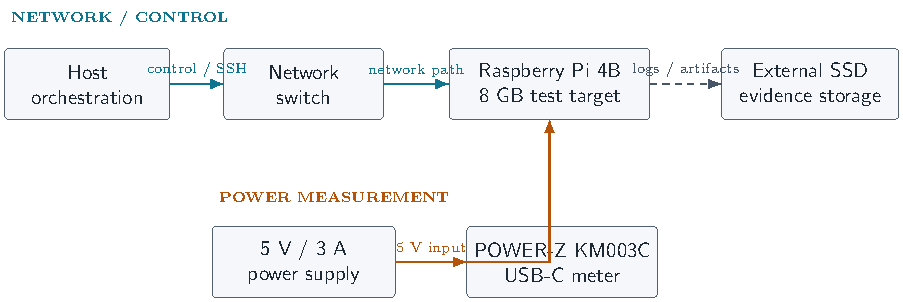
\includegraphics[width=.78\textwidth]{figures/experiment_setup_schematic.pdf}
\caption{Supply, inline POWER-Z KM003C and Raspberry Pi 4B, with Ethernet orchestration through a switch and external evidence storage. Roles are schematic; power is whole-device load-side USB input, not CPU-only power.}
\label{fig:experimentdesign}\end{figure*}

\section{Related Work}
\label{sec:relwork}
Our work sits at the intersection of edge IDS, conditional inference, model serving, and learned resource orchestration. Recent IDS research covers continual detection, heterogeneous representations, and runtime model selection~\cite{Wang2024BFSNID,AOCIDS2024,StatAvg2025,DMIDS2025}. Auto-IDaS and FEDMS show that learned or confidence-driven detector selection is operationally plausible~\cite{Lin2024AutoIDaS,Hasan2026FEDMS}, but neither a complex controller nor a cheaper operating point by itself establishes adaptive value. We therefore require comparison with the static detector actually realized by the selector and expose the full state--action map, not only visited-state occupancy.

Conditional-computation systems---including BranchyNet, adaptive network selection, MSDNet, and shallow--deep networks---escalate uncertain inputs to costlier models~\cite{Teerapittayanon2016BranchyNet,Bolukbasi2017Adaptive,Huang2018MSDNet,Kaya2019ShallowDeep}. Our fixed confidence cascade translates that idea to whole-device IDS measurement. The historical 100-row R1 regime illustrates a serving detail: 1.34\% of rows escalate across 66.76\% of windows. These historical fractions are not the corrected variable-load results; call granularity must be disclosed in each implementation.

Serving systems such as Clipper, INFaaS, and Clockwork make accuracy, latency, and cost SLOs explicit and route requests among model variants~\cite{Crankshaw2017Clipper,Romero2021INFaaS,Gujarati2020Clockwork}. We adopt their service-contract perspective but add two missing controls: a matched static action that separates routing value from model choice, and a pre-deployment audit that asks whether the declared reward permits any action reversal on validation support.

RL-based edge orchestration spans vRAN, vehicle--edge scheduling, DVFS, offloading, and QoS control~\cite{Murti2024vRAN,Zhang2024VehicleEdge,Zhang2024DVFO,Lou2024Startup,Kim2024DistributedOffload,Maleki2024QCS,Nan2026RobustDNN,Wang2025TrustOffload,Hu2025SITOff}. Tabular Q-learning and DQN are representative discrete and neural value-based controllers~\cite{Watkins1992,Mnih2015}. Our contribution is not a new RL algorithm. It combines immediate-utility screening, matched attribution, fixed factorial replay and support disclosure. The follow-up design postdates historical test inspection; fixed execution does not imply a pristine unseen-test protocol. These instruments address evaluation fragility in security ML and small-sample RL studies~\cite{Arp2022,Agarwal2021}.

\section{Compact System Model and Service Objectives}\label{sec:system}
All four frozen detectors remain resident. Before one-second window $t$, the common observation is
\begin{equation}\label{eq:state}s_t=(N_t,Q_t^-,h_{t-1},a_{t-1}),\end{equation}
where $N_t$ is current scheduled arrivals, $Q_t^-$ is FIFO carryover measured before appending current arrivals, and $h_{t-1}$ is the preceding selected path's mean posterior. Initial threat is 0.5 and prior action TinyDT. Temperature is safety telemetry only. Ground truth, cell identity, future arrivals and unselected predictions are not online features.

Static methods ignore the view. DeadlineGuard uses $N_t+Q_t^-$ and fixed calibrated MedRF p95 batch latency. RL commits a greedy frozen action. Cascade sees current-row LightLR confidence only after entry inference; this is not information given to pre-window RL. Shared load information does not imply identical computation. Rows are served FIFO in batches of at most 100. Per-batch completion times determine row deadlines; window misses and unfinished rows are separately reported. No policy updates online.

\section{Dataset-Native Data Preparation}
\label{sec:data}
\subsection{Choice of Primary Dataset}
The primary systems study uses TON-IoT~\cite{TONSource}. Its records combine IoT service telemetry, operating-system events, and networked interactions labeled with attack categories, making the dataset representative of the mixed-signal traffic that reaches an edge IDS at the service boundary rather than at the wire only. We deliberately restrict the physical dynamic-power study to a single dataset because coupling multiple encoded pipelines to one hardware campaign would confound feature dimensionality, class balance, and physical measurement; instead \cic{}~\cite{CICSource} and \nb{}~\cite{NBaIoTSource} are retained as supplementary detector and coverage audits and are not used to imply cross-dataset dynamic-power generalization.

\subsection{Frozen Preprocessing and Splits}
The TON-IoT pipeline is frozen and retains 32 native features. Imputation, scaling, and categorical encoding are fitted on training data only and applied deterministically to validation and test. The split groups unordered IP pairs so that traffic patterns are not divided across partitions; the grouping rule hashes ``$11\vert$'' concatenated with the sorted IP pair and thresholds the first sixteen SHA-256 hexadecimal digits modulo 100 (training below 60, validation 60--79, test 80--99). Training seed 11 fixes all model fits, so any single-seed conclusion is explicit rather than implied. Source-row identifiers and raw-field-string fingerprints are cross-partition disjoint, and a separate author-side encoded-float32 audit finds \emph{zero} TON-IoT train--test vector matches, which addresses a commonly-cited leakage risk in IoT IDS benchmarks~\cite{Arp2022}.

\subsection{Auxiliary Dataset Audits}
The same ledger retains dataset-native \cic{} and \nb{} pipelines with 39 and 115 native features respectively. For \cic{}, seventeen attack labels remain training-only because their capture files are too few for a defensible test split; the actual test taxonomy is a binary attack-versus-normal partition over sixteen attack categories plus benign traffic. For \nb{}, physical device identifiers are the grouping unit, giving five training, two validation, and two test devices; a post-hoc byte-level audit records that 17.3\% of \nb{} test rows share exact float32 vectors with training rows (seven distinct vectors), reflecting the sensor-repetition structure of the dataset rather than a preprocessing fault. These coverage and encoded-overlap limitations are retained rather than used to imply cross-dataset dynamic-power generality; consequently the auxiliary datasets support only static classification and replay evidence.

\subsection{Class Balance and Replay Traces}
The TON-IoT test set contains a majority attack fraction, which is common in IoT benchmarks and which we do not rebalance because the physical study measures whole-device behavior on the natural distribution. To probe operating points under controlled prevalence shifts, the supplement retains twenty static replay traces per model (fifty per dataset before deduplication), with successive phase attack fractions $\{0.05, 0.35, 0.70, 0.40, 0.10\}$ over $\{100, 100, 120, 100, 80\}$ windows. These traces do not constitute a new detector-training exercise; they resample fixed held-out pools to expose how a frozen detector's F1 and balanced accuracy behave when prevalence, not distribution, changes.

\section{Methods, Objective and Training Support}\label{sec:methods}
The four frozen detectors are depth-6 TinyDT, L2 LightLR, 25-tree depth-10 MedRF and a 64/32/16 HeavyMLP, with classifier seed 11 and threshold 0.5. No detector is refitted in the follow-up.

Current arrivals are binned as $N\leq50$, $50<N\leq100$, or $N>100$; carryover as zero, $1$--$100$, or above $100$; prior threat as below $1/3$, $[1/3,0.7)$, or at least $0.7$. Prior action changes fastest, giving $3^3\times4=108$ full states. This corrects the historical 324-state interface; the two implementations are not interchangeable.

The corrected training objective is
\begin{align}
r_t={}&0.5 B_t-0.2\bar P_t-0.2\min(c_t,1)\nonumber\\
&-\ind[c_t>1\ \mathrm{or}\ Q_{t+1}>0]-Q_{t+1}/W_t,
\end{align}
with zero pending fraction for zero work. $B$ is balanced accuracy, $W=N+Q^-$ and $c$ is completion seconds. Power is min--max normalized historical TON static mean power. Simulated completion uses the newly calibrated warm-input p95 per 100 rows. These are training surrogates, not measurements of variable-load energy or causal thermal response. Temperature has no reward component.

There are 25 frozen policies: Q full/minus-arrival/minus-threat/minus-previous-action for five seeds (2003, 2011, 2017, 2027, 2029), and five full DQN policies. Each uses 1,000 episodes of 500 windows. Original policy hyperparameters are retained; last-episode checkpoints alone are eligible. Full-policy seed selection maximizes summed validation reward, ties choosing the lowest seed. Selected policies are Q seed 2011 and DQN seed 2003. No physical/test result changes selection. Workload traces and prediction pools are hash-bound.

The fixed surrogate has zero carryover throughout. Queue ablation is NOT IDENTIFIABLE/NOT EXECUTED, not evidence of robustness. Validation resamples an existing validation pool rather than creating independent examples. Full-source and transition archives disclose this limitation.

\subsection{Immediate Pairwise Preferences, Not Policy Optimality}
For fixed-support immediate utility $U_a=w_DD_a-C_a$, $w_D>0$, action $a$ beats $b$ iff $D_a-D_b>(C_a-C_b)/w_D$. Strict preference reversals require the threshold to lie strictly between attainable differences. This algebra applies only to the declared instantaneous costs and support. It does not determine transition dynamics, long-horizon return, a globally optimal policy, or inevitable learned collapse. The retrospective historical audit finds TinyDT-favouring windows and cannot prove global LightLR optimality or execution before test inspection. Load-dependent cost terms require a support-conditioned audit; historical numeric thresholds are not transferred to the corrected objective.

External denominators such as an idle-relative power budget and latency SLO can make objectives interpretable independently of pool extrema. This is a design rule, not an experimentally established benefit of a different reward, which we do not tune here.

\section{Measurement and Statistical Protocol}\label{sec:eval}
The corrected follow-up retains six methods and the previously fixed ten-block order. Each formal run has 60 seconds of preceding instrumented idle and 500 one-second workload windows: nine load--prevalence cells, 50 windows each, followed by 50 recovery windows. Rows are repeated presentations from fixed pools, not fresh network attacks. Ground-truth labels are used for post-run metrics, never online control.

One Raspberry Pi 4B 8 GB is powered through POWER-Z KM003C HW 2.4/FW 2.0.6. All detectors remain resident. Wi-Fi stays enabled and Ethernet orchestration is pinned; these platform conditions are disclosed rather than attributed to scheduler savings. The meter is not independently laboratory calibrated. Nominal 1-Hz samples retain raw frames, signed current, voltage and request/receive times. With $P_i=V_i(-I_i)$, energy is
\begin{equation}\label{eq:trap}
E=\sum_i\tfrac12(P_i+P_{i+1})(\tau_{i+1}-\tau_i).
\end{equation}
This is whole-device load-side input, not CPU-only joules or wall energy. No missing samples are filled.

Continuous process-aware CPU accounting brackets explicitly allowed worker PID/starttime counters with global busy/total counters. Its conservative external fraction is $\max(0,B_{\rm upper}-A)/T_{\rm lower}$, including unattributed kernel/IRQ and transient work. Fractions above 5\%, intervals above 1.5 seconds, missing coverage, thermal/throttle, clock, disk or meter failures reject the attempt. Replacements require explicit authorization; invalid bytes remain archived. Monitor cadence was repaired after the second interruption without relaxing either threshold.

Physical statistics use paired blocks, never rows/windows/power frames. For block differences $d_b$, report $\bar d\pm t_{.975,n-1}s_d/\sqrt n$. Raw energy is primary. Also report preceding-idle-adjusted energy $E_b-\bar P_{{\rm idle},b}\Delta\tau_b$ and corresponding power. All pairs and A/B/C sets are retained, with nominal unadjusted intervals; there is no equivalence margin or result-driven exclusion. Historical studies are never pooled with these ten blocks.

Authors report 197,922 integrity/accounting checks and a separate 12.5-million-transition audit. These are author-side results, not independent acceptance. External ZIP/raw-log review remains incomplete due to the review environment's inability to open attachments. This manuscript is a working revision, not an independently certified submission release.

\section{Static Operating Points and Historical Context}\label{sec:staticresults}
The frozen detector pool predates the follow-up. Table~\ref{tab:classification} reports its original TON-IoT classification evaluation, not a pooled average of physical blocks. MedRF's aggregate held-out BA advantage over LightLR is approximately 0.0140, a descriptive post-freeze statistic rather than a statewise attainability bound. At prevalence $p$, recall $r$ and FPR $f$,
\begin{equation}F1=\frac{2pr}{p(1+r)+(1-p)f}.
\end{equation}
Thus F1 alone can conceal normal-class errors; recall and FPR accompany energy throughout.
\begin{table}[t]\centering\small
\caption{Historical frozen TON-IoT classification at threshold 0.5, separate from new physical-block statistics.}\label{tab:classification}
\begin{tabular}{lrrrr}\toprule Model & F1 & Recall & BA & FPR (\%)\\\midrule
\tableinput{tables/ton_classification_rows}
\bottomrule\end{tabular}\end{table}

Fifteen original static-power segments characterize one Pi and resident TON detectors at 100 encoded rows/s. Idle averages 2.335 W; active means span approximately 2.347--2.397 W. Those static powers are training proxies, not new three-dataset measurements. The corrected same-runtime latency calibration uses training-origin warm input; it excludes a full closed-loop controller/transport energy measurement.

The original 40-run campaign and P1A motivated including Static-LightLR when learned policies selected it. Historical DQN versus Static-LightLR was +4.525 J in P1A, but neither that observation nor isolated timing attributes the difference to CPU computation. P1B measures approximately 10.8 microseconds per Q decision and 1.567 ms per DQN decision on its declared support, not joules. CFSM's historical switching does not establish useful switching. Historical R1 cascade call granularity is likewise a different, 100-row serving regime, not the corrected variable-load trade-off.

P1C--P1E remain separately archived. Fifteen minus-temperature/queue/arrival runs remove constant training coordinates and therefore do not establish robustness to changes in those dimensions. Historical R2's queue timing/normalization and unequal arrival visibility invalidate its use as an interface-matched RL versus DeadlineGuard comparison. These qualifications change interpretation without rewriting past executed bytes. No historical energy, confusion count, failed attempt or seed is pooled into the new ten-block array.

\section{Corrected Follow-up: Matched Static Attribution}\label{sec:dynamicresults}
The main current comparison is the November follow-up, not historical R2. It contains 60 accepted 500-second runs: six methods in ten trace-matched blocks. Classifiers, threshold 0.5 and held-out pool are unchanged. New policies were trained on training caches and selected by validation before deployment. Historical test outcomes had already been inspected before this follow-up was designed; it is not a new untouched-test experiment.

\subsection{Realized Actions and Feasibility}
In all 5,000 windows per method, Q, DQN and Static-LightLR use LightLR; DeadlineGuard and Static-MedRF use MedRF. Their within-block detection summaries coincide. No method records a deadline-miss window. Thus neither learned policies nor DeadlineGuard demonstrate useful load-conditioned switching here. Historical Tabular-Q TinyDT behavior is not reproduced under the corrected interface. This does not establish global policy optimality.

\subsection{Paired Energy and Detection}
DQN minus Static-LightLR is +0.599 J, paired Student-$t$ 95\% CI $[-4.119,5.317]$ J. Q minus Static-LightLR is +0.246 J $[-4.055,4.547]$ J. Neither contrast resolves energy savings. No equivalence margin was declared, so an interval crossing zero does not establish equivalence.

Cascade minus Static-MedRF is $-12.064$ J $[-16.548,-7.580]$ J. Mean F1 changes by $-0.0004457$ ($-0.0446$ percentage points), recall by $-0.2411$ pp and FPR by $-0.1534$ pp. This is a detection--energy trade-off, not a free improvement. The historical 1.373-pp DeadlineGuard trade-off is not a new-study result.
Tables~\ref{tab:followup} and~\ref{tab:sensitivity} retain method summaries and all registered sensitivity endpoints for the key contrasts.
\begin{table*}[t]\centering\small
\caption{Corrected follow-up: means over ten blocks; energy mean $\pm$ sample SD. Each method has zero deadline-miss windows. No historical experiment is pooled.}\label{tab:followup}
\begin{tabular}{lrrrr}\toprule Method & Energy (J) & F1 & Recall (\%) & FPR (\%)\\\midrule
Cascade & $1480.56\pm9.28$ & 0.99017 & 99.408 & 1.364\\
DQN & $1440.57\pm8.73$ & 0.97633 & 96.680 & 1.351\\
DeadlineGuard & $1492.11\pm10.75$ & 0.99062 & 99.649 & 1.517\\
Static-LightLR & $1439.97\pm9.95$ & 0.97633 & 96.680 & 1.351\\
Static-MedRF & $1492.63\pm10.58$ & 0.99062 & 99.649 & 1.517\\
Q & $1440.21\pm9.57$ & 0.97633 & 96.680 & 1.351\\
\bottomrule\end{tabular}\end{table*}
\begin{table*}[t]\centering\footnotesize
\caption{All registered block sets, nominal paired 95\% intervals. A: all blocks; B: exclude 1; C: exclude 1 and 5. Energy differences are first minus second; adjusted energy subtracts preceding idle power times observed duration.}\label{tab:sensitivity}
\begin{tabular}{llllrr}\toprule Set & Contrast & Endpoint & $n$ & Difference (J) & 95\% CI (J)\\\midrule
A & Cascade--Static-MedRF & Raw & 10 & -12.064 & $[-16.548,-7.580]$\\
B & Cascade--Static-MedRF & Raw & 9 & -11.717 & $[-16.748,-6.686]$\\
C & Cascade--Static-MedRF & Raw & 8 & -11.359 & $[-17.129,-5.588]$\\
A & Cascade--Static-MedRF & Adjusted & 10 & -16.089 & $[-26.719,-5.460]$\\
B & Cascade--Static-MedRF & Adjusted & 9 & -16.412 & $[-28.498,-4.326]$\\
C & Cascade--Static-MedRF & Adjusted & 8 & -14.862 & $[-28.287,-1.438]$\\
A & DQN--Static-LightLR & Raw & 10 & 0.599 & $[-4.119,5.317]$\\
B & DQN--Static-LightLR & Raw & 9 & 1.045 & $[-4.207,6.298]$\\
C & DQN--Static-LightLR & Raw & 8 & 2.376 & $[-2.580,7.333]$\\
A & DQN--Static-LightLR & Adjusted & 10 & 0.974 & $[-9.667,11.615]$\\
B & DQN--Static-LightLR & Adjusted & 9 & 2.117 & $[-9.647,13.882]$\\
C & DQN--Static-LightLR & Adjusted & 8 & 3.775 & $[-9.161,16.711]$\\
A & Q--Static-LightLR & Raw & 10 & 0.246 & $[-4.055,4.547]$\\
B & Q--Static-LightLR & Raw & 9 & 0.489 & $[-4.372,5.350]$\\
C & Q--Static-LightLR & Raw & 8 & 2.235 & $[-0.934,5.404]$\\
A & Q--Static-LightLR & Adjusted & 10 & -4.793 & $[-17.147,7.562]$\\
B & Q--Static-LightLR & Adjusted & 9 & -2.694 & $[-15.693,10.306]$\\
C & Q--Static-LightLR & Adjusted & 8 & 1.593 & $[-8.224,11.410]$\\
\bottomrule\end{tabular}\end{table*}


\subsection{Interruptions and Sensitivity}
Two rejected attempts are preserved: block 1 Static-LightLR exceeded 5\% external CPU, coincident with man-db maintenance; block 5 Cascade's idle failed the 1.5-second monitor-gap limit. Accepted runs were retained; explicitly authorized new IDs recover only the interrupted portion. Both blocks span periods. Idle subtraction does not guarantee elimination of temporal confounding.

The derived monitor waits relative to actual sampling time rather than adding one second after processing, and retains rejected snapshots. CPU accounting, 5\% and 1.5-second limits, service loop and policies are unchanged. The old rejected gap lacks its right snapshot; exact duration is unavailable. Both executed source versions are preserved.

We report A: all ten blocks; B: exclude block 1 ($n=9$); C: exclude blocks 1 and 5 ($n=8$), each with raw and preceding-idle-adjusted results. Registration timestamps are actual campaign-time additions, not backdated original preregistration. All method pairs are retained; nominal intervals are not multiplicity-adjusted and no favourable set is selected.

\subsection{Historical Evidence Boundary}
The original study, P0/P1 and old R1/R2 are not pooled. Old R2 used mismatched arrival timing and post-append queue encoding; its TinyDT behavior is an implementation diagnostic, not an interface-matched algorithm comparison. Constant-coordinate ablations do not establish load/queue/thermal robustness. The historical DQN block-4 excursion lacked the later process-aware gate; no precise external-process joule attribution follows. R3 remains NOT EXECUTED; timing is not controller-only energy. Threshold diagnostics do not replace frozen threshold=0.5 results.

\section{Discussion}\label{sec:discuss}
The corrected comparison distinguishes static detector choice from conditional value. Q/DQN realize LightLR; neither shows resolved energy savings against directly deploying it. DeadlineGuard realizes MedRF, so this experiment does not demonstrate a switching benefit or superiority over an infeasible static control. The cascade's lower energy relative to MedRF accompanies lower recall and F1 and lower FPR. Its current-row confidence access and call granularity differ from pre-window model selection; it is not a universal architecture ranking.

Historical interface defects, constant-coordinate ablations and external interference explain why implementation auditing must precede algorithm-level interpretation. They do not justify erasing old evidence or rerunning until a preferred ordering emerges. Matching state meanings does not match state distributions: queue remained constant in training. The immediate utility preference calculation is useful as a reward audit but is not a theorem explaining long-horizon policy collapse. Raw and idle-adjusted results, recovered-block sensitivities, exact executed versions and real registration times are all necessary to constrain attribution.

\section{Limitations}\label{sec:limits}
Ten paired blocks on one Pi do not estimate device/site/fleet variation. Only TON-IoT has dynamic physical testing; no TON power proxy is represented as measured CICIoT2023 or N-BaIoT cost. Scheduled encoded-feature replay excludes packet capture and encoding. Historical test outcomes were inspected before the follow-up design; validation-only policy selection does not make the test historically unseen. Training backlog is constant; no queue-adaptation or thermal capability is claimed. Historical constant-temperature conventions were not action-attributable measurements.

Blocks 1 and 5 span recovery periods and monitoring versions. Both are retained and both exclusion rules disclosed, but adjustment cannot prove removal of all drift. The old failed monitor interval lacks a right snapshot, so its exact duration is unavailable. Controller-only R3 was not executed. Neither timing nor assumed CPU watts resolves controller joules. Nominal paired intervals are not multiplicity-adjusted and do not establish equivalence. Author validation and partial independent review have different scopes. No final submission-readiness claim is made while consistency and independent review remain open.

\section{Conclusion}\label{sec:conclude}
Under the corrected common interface, frozen Q and DQN realize Static-LightLR while DeadlineGuard realizes Static-MedRF. The measured RL/static contrasts do not resolve savings and do not prove equivalence. Cascade exhibits a specific detection--energy trade-off rather than a free adaptive improvement. The transferable result is the need to separate model operating points, causal information, training support, objective assumptions and measurement interference. Historical implementation outcomes, corrected follow-up measurements and independent-review scope must remain distinct.

\bibliographystyle{IEEEtran}
\bibliography{references}
\end{document}
